\renewcommand{\NomeBloco}{\emph{Inversor}}
\renewcommand{\NomeBlocoNoIt}{Inversor}
\renewcommand{\NomePTab}{tab_\NomeBlocoNoIt}
\renewcommand{\NomeSTab}{tab_\NomeBlocoNoIt2}
\renewcommand{\NomePFig}{fig_\NomeBlocoNoIt}
\renewcommand{\NomeSFig}{fig_\NomeBlocoNoIt2}
\renewcommand{\NomeTTab}{tab_\NomeBlocoNoIt3}

\section{\NomeBloco}
\label{inversor1}

O bloco \NomeBloco{} tem a finalidade de receber uma entrada digital, e colocar o n\'ivel l\'ogico invertido na sa\'ida. A \autoref{\NomePTab} indica a Tabela Verdade do bloco.

\begin{table}[htbp]

\caption{Tabela Verdade do bloco \NomeBloco}%
\label{\NomePTab}
\centering
\begin{tabular}{cc}
    \toprule
    Entrada & Saída \\
    \midrule \midrule
    0 & 1 \\
    \midrule
    1 & 0 \\
\bottomrule

\end{tabular}
\fonte{Produzido pelo autor.}
\end{table}

O bloco apresenta as defini{\c c}\~oes de sinais de entrada e sa\'ida referidos na \autoref{\NomeSTab}.

\begin{table}[htbp]
\caption{Sinais do bloco \NomeBloco}
\label{\NomeSTab}
\centering
\begin{tabular}{ccl}

    \toprule
    Sinal & Tipo    & Descri{\c c}\~ao        \\
    \midrule \midrule
    In    & Entrada & Sinal de Entrada \\
    \midrule
    Out   & Saída   & Sinal de Sa\'ida   \\
    \bottomrule
\end{tabular}
\legend{Fonte: Produzido pelo autor}
\end{table}

O circuito projetado para o bloco \'e demonstrado na \autoref{\NomePFig}.

\begin{figure}[htb]
 \label{NomePFig}
 \centering
  \begin{minipage}{0.4\textwidth}
    \centering
    \caption{Circuito CMOS projetado para o bloco \NomeBloco} \label{\NomePFig}
    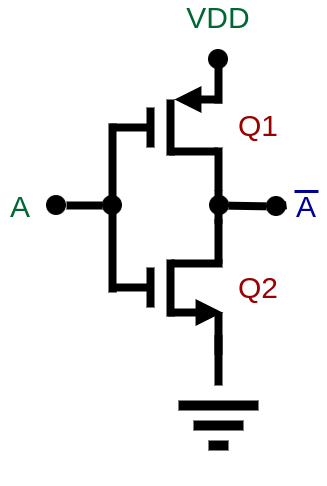
\includegraphics[scale=0.3]{Circuitos/NOT.png}
    \legend{Fonte: Produzido pelo autor}
  \end{minipage}
  \hfill
  \begin{minipage}{0.4\textwidth}
    \centering
    \caption{Representa{\c c}\~ao em bloco do \NomeBloco} \label{NomeSFig}
    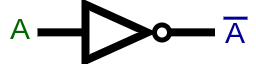
\includegraphics[scale=0.3]{Circuitos/NOT_block.png}
    \legend{Fonte: Produzido pelo autor}
  \end{minipage}
\end{figure}

Os transistores utilizados no bloco \NomeBloco{} apresentam os par\^ametros mostrados na \autoref{\NomeTTab}.

\begin{table}[htbp]
\caption{Transistores do Bloco \NomeBloco}
\label{\NomeTTab}
\centering
\begin{tabular}{ccccc}
\toprule
Transistor & W ($\mu$m)  & L ($\mu$m)           & M (n° dispositivos) & S (n° dispositivos)\\
\midrule \midrule
Q1 & 1,2 & 0,18 & 1 & 1\\
\midrule
Q2 & 0,6 & 0,18 & 1 & 1\\
\bottomrule
\end{tabular}
\legend{Fonte: Produzido pelo autor}
\end{table}